\documentclass[tikz,border=0pt]{standalone}
\usepackage[utf8]{inputenc}
\usepackage{csquotes}
\usepackage{xcolor}
\usepackage{graphicx}
\usepackage{pgffor}
\usepackage{listings}
\usepackage{array}
\usepackage{fontawesome}
\usepackage{amsmath}

\lstset{
    basicstyle=\ttfamily\fontsize{6}{8}\selectfont,
    breaklines=true,
    % backgroundcolor=\color{black},
    keywordstyle=\color{pink},
    commentstyle=\color{blue},
    stringstyle=\color{white},
    showstringspaces=false,
    frame=none,
    xleftmargin=0.6cm,
    xrightmargin=0.6cm
}

\begin{document}
\begin{tikzpicture}
\useasboundingbox (0,0) rectangle (10.8,10.8);

% Hintergrund in Schwarz
\fill[black] (0,0) rectangle (10.8,10.8);

% Zufällige Einsen und Nullen verteilen
\foreach \i in {1,...,5000} {
    \node[text=green, opacity=0.1, font=\ttfamily\fontsize{5}{6}\selectfont] at (rand*10.8, rand*10.8) {\pgfmathtruncatemacro{\random}{round(rand)}\random};
}

% \fill[red, opacity=0.1] (0.05,5.95) rectangle (10.75,10.75);
% \draw[red, thin] (0.05,5.95) rectangle (10.75,10.75); % 45% Höhe
\node[red, anchor=north west, font=\ttfamily\bfseries\fontsize{8}{9}\selectfont] at (0.1,10.65) {NVD DB Update {\Large{ CVE-2012-1856} - \textbf{Score:}{\Large{ 8.8 }}}};
% % ------------------------------------------------------------------------------------------------------------------------------
% \node[red, anchor=north west, font=\ttfamily\fontsize{8}{9}\selectfont, text width=10.6cm, align=center] at (0.1,10.25) {
% \newline
% \newline
% \newline
% If you want to succeed in penetration testing and cybersecurity, learn at least:
% \newline
% };
% ------------------------------------------------------------------------------------------------------------------------------
\fill[green, opacity=0.1] (0.05,1.15) rectangle (10.75,10.75);
\draw[green, thin] (0.05,1.15) rectangle (10.75,10.75); % 45% Höhe
% \node[green, anchor=north west, font=\ttfamily\bfseries\fontsize{8}{9}\selectfont] at (0.1,5.65) {Solution:};
% ------------------------------------------------------------------------------------------------------------------------------
\node[green, anchor=north west, font=\ttfamily\fontsize{8}{9}\selectfont, text width=10.6cm, align=center] at (0.1,10.25) {
\textbf{Components:}
\begin{scriptsize}
\begin{lstlisting}
 microsoft office 2007
 microsoft sql server 2000
 microsoft office 2003
 microsoft sql server 2005
 microsoft visual foxpro 8.0
 microsoft commerce server 2002
 microsoft visual foxpro 9.0
 microsoft office 2010
 microsoft sql server 2008
 microsoft host integration server 2004
 microsoft commerce server 2007
 microsoft visual basic 6.0
 microsoft commerce server 2009
 microsoft office web components 2003
\end{lstlisting}
\end{scriptsize}
\textbf{Description:}
\begin{scriptsize}
\begin{lstlisting}
The TabStrip ActiveX control in the Common Controls in MSCOMCTL.OCX in Microsoft Office 2003 SP3, Office 2003 Web Components SP3, Office 2007 SP2 and SP3, Office 2010 SP1, SQL Server 2000 SP4, SQL Server 2005 SP4, SQL Server 2008 SP2, SP3, R2, R2 SP1, and R2 SP2, Commerce Server 2002 SP4, Commerce Server 2007 SP2, Commerce Server 2009 Gold and R2, Host Integration Server 2004 SP1, Visual FoxPro 8.0 SP1, Visual FoxPro 9.0 SP2, and Visual Basic 6.0 Runtime allows remote attackers to execute arbitrary code via a crafted (1) document or (2) web page that triggers system-state corruption, aka "MSCOMCTL.OCX RCE Vulnerability."
\end{lstlisting}
\end{scriptsize}
\textbf{Main problems:}
\begin{scriptsize}
\begin{lstlisting}
-1 no CWE Description available

\end{lstlisting}
\end{scriptsize}
};
% ------------------------------------------------------------------------------------------------------------------------------
\draw[green, thin] (0.05,0.05) rectangle (10.75,1.05); % 10% Höhe
% \node[green, anchor=north west, font=\ttfamily\bfseries\fontsize{5}{6}\selectfont] at (0.1,0.95) {Contact:};

% Tabelle 2x2 im Contact Block
\node[green, anchor=north west, font=\ttfamily\fontsize{8}{9}\selectfont, text width=10.6cm] at (0.1,0.95) {
\begin{tabular}{@{}p{4.8cm}@{}p{5cm}@{}}
\faGlobe\ https://cybersword.tech & \faLinkedin\ www.linkedin.com/in/cybersword-tech \\
\faInstagram\ ph1sher & \faTwitter\ @davidwowa \\
\end{tabular}
};
\end{tikzpicture}
\end{document}